\section{IR with Low-Rank Preconditioner}
\label{sec:low_rank}

For evaluation of iterative refinement with low-rank preconditioners, it was necessery to adapt the experimental settings to fit this new environment. Instead of ordinary random matrices, structured random matrices were used, as those guarantee the existence of low-rank approximations with adjustable accuracy based on the chosen rank. In order to account for the higher performance of such representations, $4096 \times 4096$ element matrices were added to the test set. Each test matrix was created with a laplacian kernel from a randomized, ordered vector. A similar vector was used for the accurate solution $\hat{x}$ and the right hand-side $b$ was calculated via $b = A\hat{x}$. The condition numbers of these matrices were set by adjusting their absolute values and the resulting quantities were then used as the input for the solver. Both GMRES- and LU- based IR procedures were adapted to first create a hierarchical representation of $A$ and the use the LU factors obtained from this matrix during the iteration steps. The accuracy of the hierarchical representation (denoted as $\epsilon$) was controlled via the rank, trying to find settings close to $\{10^{-2}, 10^{-4}, 10^{-6}, 10^{-8}\}$ (the reciprocals of the evaluated condition numbers).
Both methods were evaluated with the precisions set to: $u_f= double$, $u= double$, $u_r= quadruple$.
Note that even though the factorization precision is double, the actual accuracy is limited by the parameter $\epsilon$ and a single solve with those LU factors cannot expect to achieve an error smaller than this threshold. The result of the error analysis for different test-matrices with a size of $512 \times 512$ are displayed in Figures~\hyperref[fig:lrir1]{\ref{fig:lrir1}} - \hyperref[fig:lrir4]{\ref{fig:lrir4}}.

\begin{figure}
\centering
\begin{subfigure}{.5\textwidth}
  \centering
  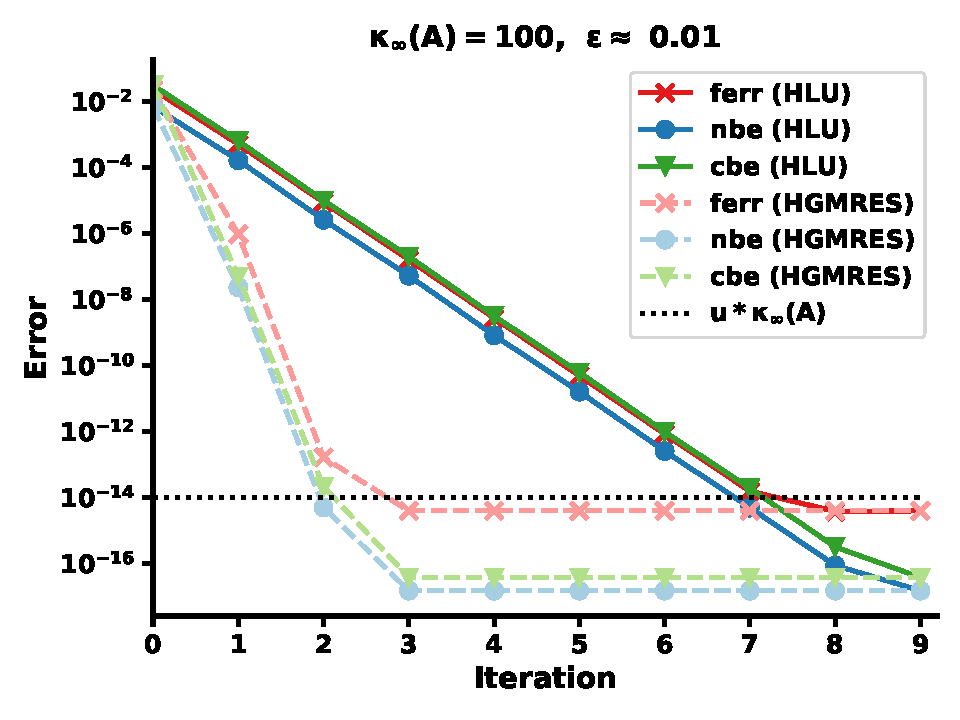
\includegraphics[width=\linewidth]{chapters/5_experiments/figures/LR512e0_0.pdf}
  \caption{$\epsilon \approx 10^{-2}$}
  \label{fig:lrir1_1}
\end{subfigure}%
\begin{subfigure}{.5\textwidth}
  \centering
  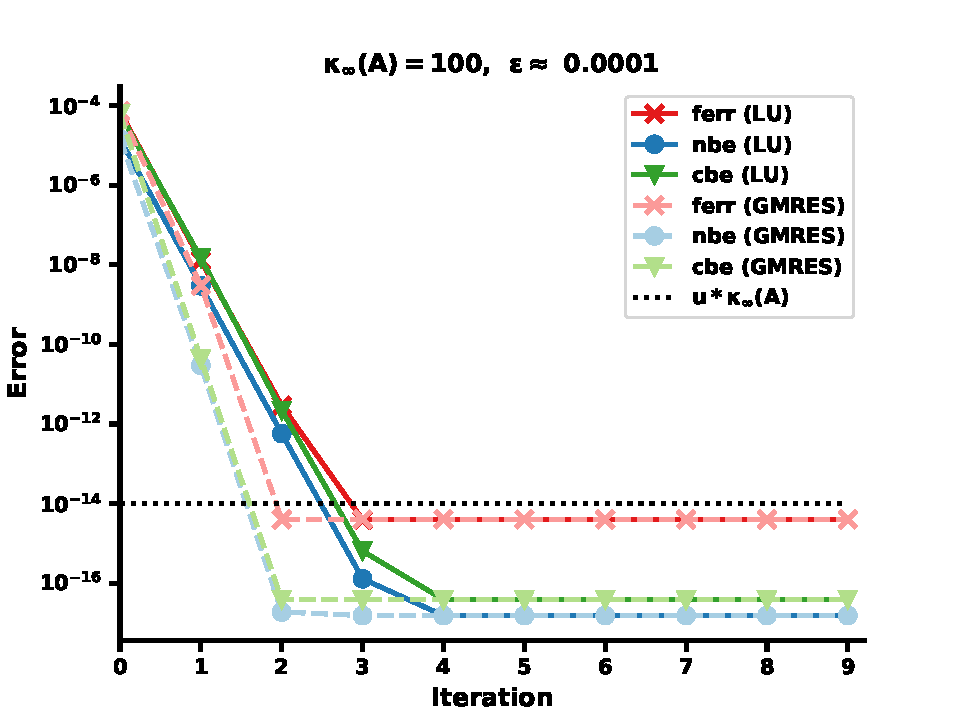
\includegraphics[width=\linewidth]{chapters/5_experiments/figures/LR512e0_1.pdf}
  \caption{$\epsilon \approx 10^{-4}$}
  \label{fig:lrir1_2}
\end{subfigure}
\caption[Low-Rank IR 1]{LU- and GMRES-based IR for a matrix $A$ with $\kappa_\infty(A) \approx 10^2$.}
\label{fig:lrir1}
\end{figure}

\begin{figure}
\centering
\begin{subfigure}{.5\textwidth}
  \centering
  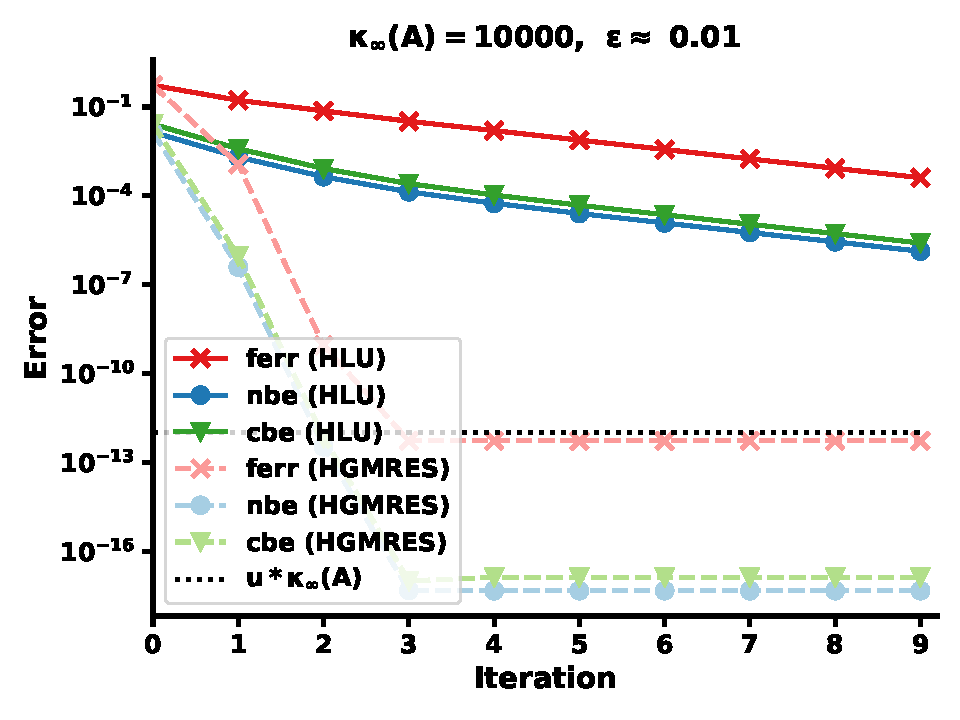
\includegraphics[width=\linewidth]{chapters/5_experiments/figures/LR512e1_0.pdf}
  \caption{$\epsilon \approx 10^{-2}$}
  \label{fig:lrir2_1}
\end{subfigure}%
\begin{subfigure}{.5\textwidth}
  \centering
  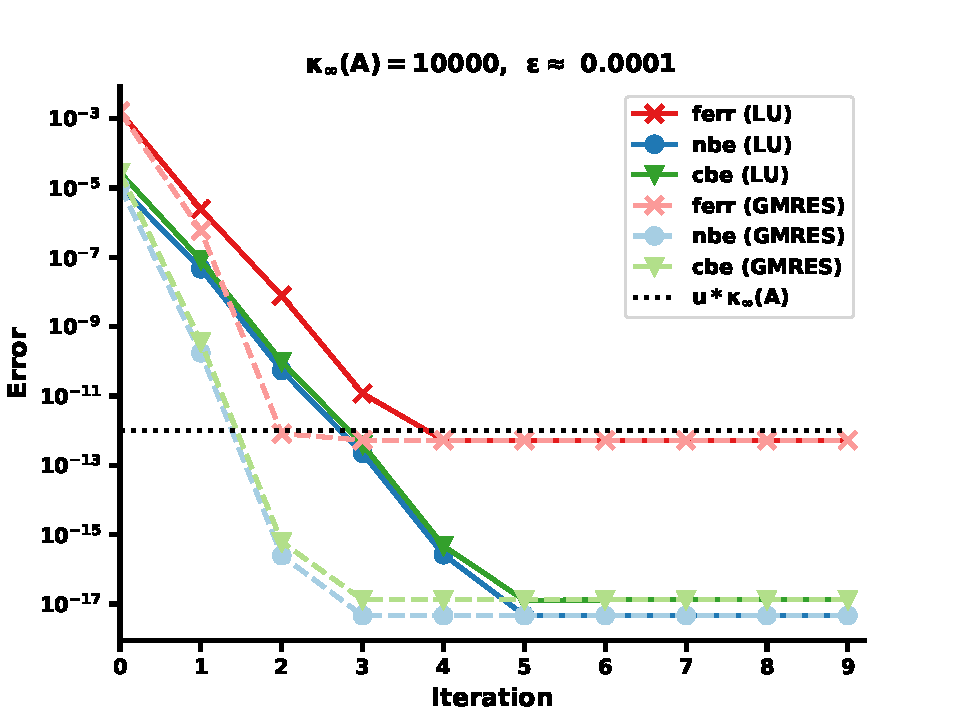
\includegraphics[width=\linewidth]{chapters/5_experiments/figures/LR512e1_1.pdf}
  \caption{$\epsilon \approx 10^{-4}$}
  \label{fig:lrir2_2}
\end{subfigure}
\caption[Low-Rank IR 2]{LU- and GMRES-based IR for a matrix $A$ with $\kappa_\infty(A) \approx 10^4$.}
\label{fig:lrir2}
\end{figure}

\begin{figure}
\centering
\begin{subfigure}{.5\textwidth}
  \centering
  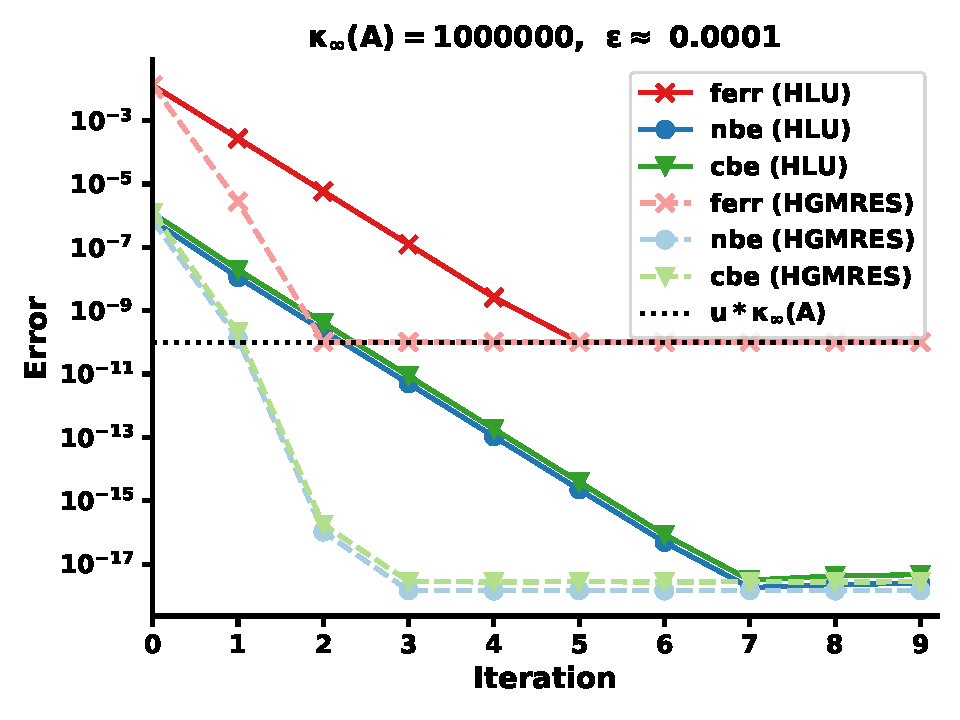
\includegraphics[width=\linewidth]{chapters/5_experiments/figures/LR512e2_0.pdf}
  \caption{$\epsilon \approx 10^{-4}$}
  \label{fig:lrir3_1}
\end{subfigure}%
\begin{subfigure}{.5\textwidth}
  \centering
  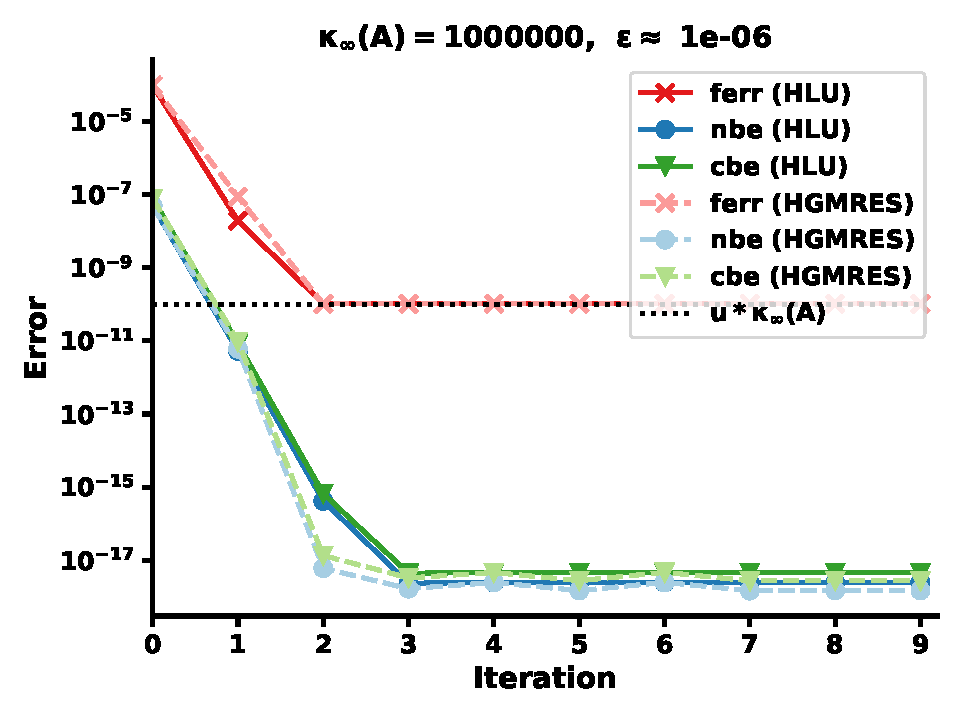
\includegraphics[width=\linewidth]{chapters/5_experiments/figures/LR512e2_1.pdf}
  \caption{$\epsilon \approx 10^{-6}$}
  \label{fig:lrir3_2}
\end{subfigure}
\caption[Low-Rank IR 3]{LU- and GMRES-based IR for a matrix $A$ with $\kappa_\infty(A) \approx 10^6$.}
\label{fig:lrir3}
\end{figure}

\begin{figure}
\centering
\begin{subfigure}{.5\textwidth}
  \centering
  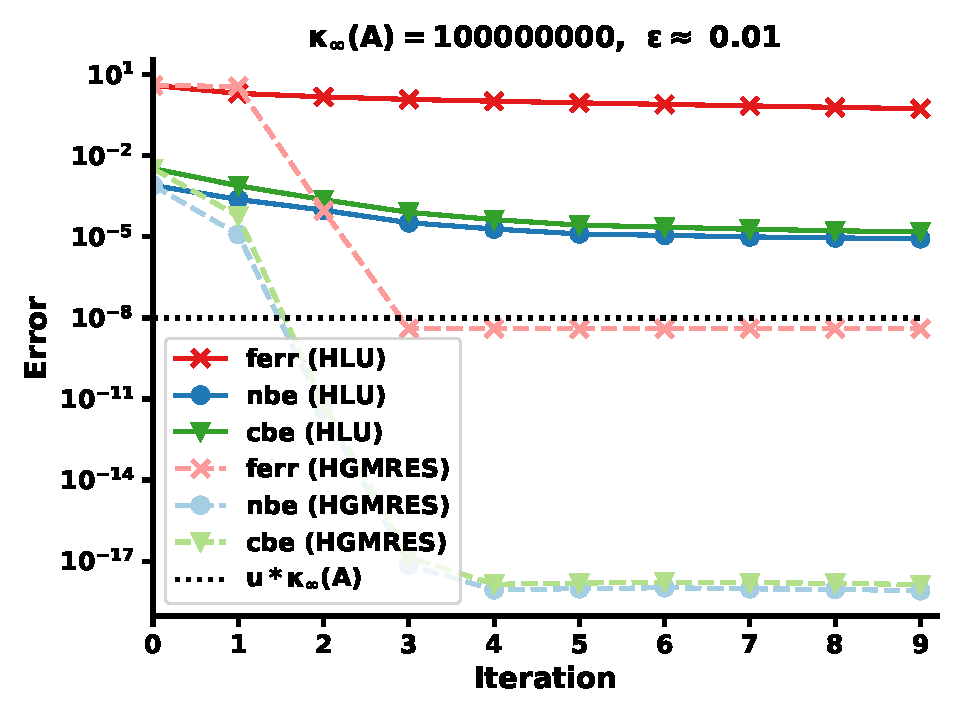
\includegraphics[width=\linewidth]{chapters/5_experiments/figures/LR512e3_0.pdf}
  \caption{$\epsilon \approx 10^{-2}$}
  \label{fig:lrir4_1}
\end{subfigure}%
\begin{subfigure}{.5\textwidth}
  \centering
  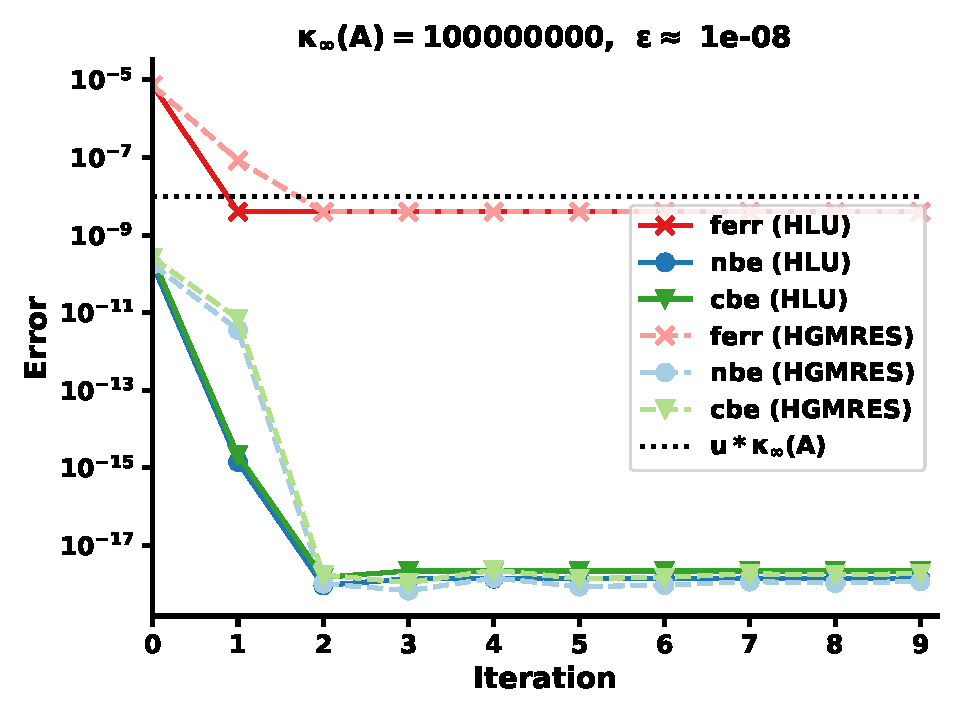
\includegraphics[width=\linewidth]{chapters/5_experiments/figures/LR512e3_1.pdf}
  \caption{$\epsilon \approx 10^{-8}$}
  \label{fig:lrir4_2}
\end{subfigure}
\caption[Low-Rank IR 4]{LU- and GMRES-based IR for a matrix $A$ with $\kappa_\infty(A) \approx 10^8$.}
\label{fig:lrir4}
\end{figure}

First we note that the hierarchical representation seems to help with the condition number, achieving convergence in all cases if $\epsilon$ is small enough. Even for the case $\kappa\infty(A)=10^8$, where we observed breakdown of LU-based IR in the three precision setting (see Section~\hyperref[sec:low_precision_ir]{\ref{sec:low_precision_ir}}), the low-rank LU iterative refinement process still converges. However, while both norm-wise and component-wise backward errors can be reduced down to working precision, the accuracy of the forward error seems to be limited. Based on the conducted experiments it seems to be restricted by the product of the working precision $u$ and the condition number $\kappa\infty(A)$, which is represented as a dashed line in the plots. Based on the numerical results obtained, this seems to be an accurate estimation and is, most interestingly, independent from the accuracy of the factorization $\epsilon$.

While it might not be the deciding factor for convergence itself, the number of iterations (and thus the convergence speed) are highly dependent on $\epsilon$. This can be observed quite clearly in Figures~\hyperref[fig:lrir2_1]{\ref{fig:lrir2_1}} \& \hyperref[fig:lrir2_2]{\ref{fig:lrir2_2}}, where LU-based iterative refinement converges in 4 steps with $\epsilon = 10^{-4}$ while more than $10$ iterations would be necessary for $\epsilon = 10^{-2}$. For the case of GMRES-based IR, the connection is less obvious, but still observable. Despite that, the influence on the number of inner GMRES iterations seems to be limited without any immediately visible correlations. Further research would be necessary in order to investigate this behaviour.

Examining the impact of the matrix size on the error and number of iterations, results similar to the case of iterative refinement in three precisions can be obtained. Both backwards errors, the forward error and the number of iterations necessary remain constant (apart from slight fluctuations possibly due to the differences in $\epsilon$). This behaviour is demonstrated in Figure~\hyperref[fig:lr_ir_size]{\ref{fig:lr_ir_size}}, showing the errors for an increasing matrix size $n$. LU-based IR needs exactly five steps in most cases (the exceptions are $n = \{1024, 2048\}$, where four iterations are sufficient), while GMRES finishes in just three steps every time (although the number of inner iterations increases). However, this growth in the number of inner iterations is expected when increasing the dimensionality of the problem, since it is proportional to the number of subspaces potentially searched by GMRES. 

\begin{figure}[h]
    \centering
    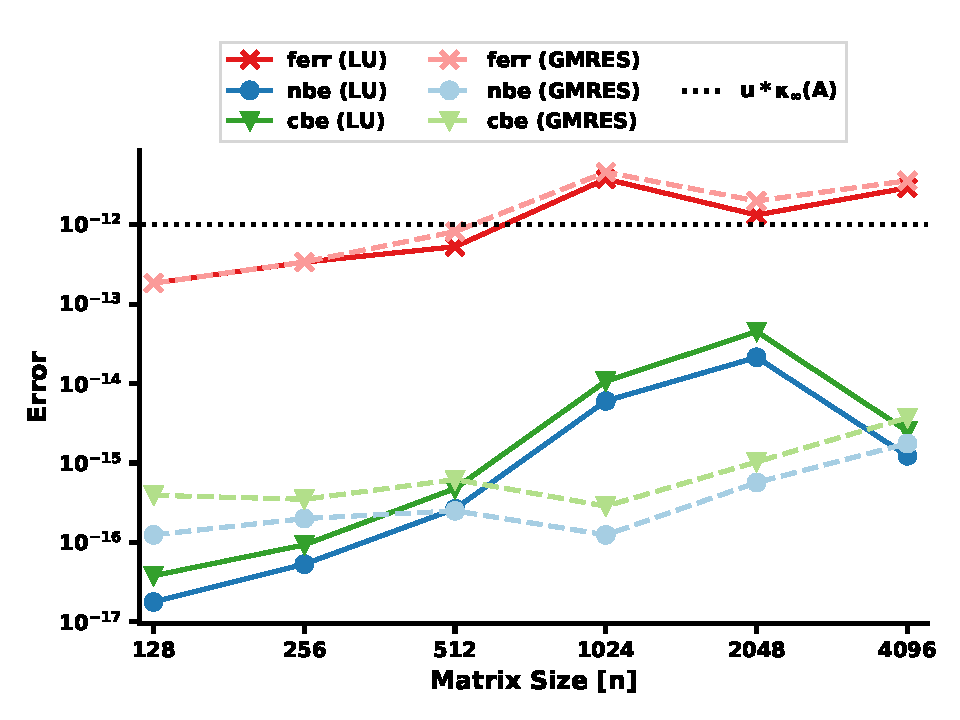
\includegraphics[width=0.7\linewidth]{chapters/5_experiments/figures/LR_size.pdf}
    \caption[Low-Rank IR - Matrix Size]{Low-rank IR applied to various matrix sizes. $\kappa_\infty(A) \approx 10^4$ and $\epsilon \approx 10^{-4}$ for all matrices. The errors remain relatively constant.}
    \label{fig:lr_ir_size}
\end{figure}

Nonetheless, it is worth investigating, as it is an essential criterion for the efficiency of GMRES-based IR, potentially causing a large runtime. As explained in Section~\hyperref[sec:preconditioners]{\ref{sec:preconditioners}} fast convergence of Krylov-subspace methods depends on a suitable preconditioner. In this context, the approximate LU factors obtained via the hierarchical factorization are used and it is worthwhile to evaluate their influence. For assessing the benefits of this preconditioning, we compare the performance of GMRES-based IR for two different preconditioners:
\begin{itemize}
    \item \textit{Diagonal preconditioner}: The diagonal elements of $A$ are used as a preconditioner (also known as Jacobi preconditioner).
    \item \textit{LU preconditioner}: Using the approximate LU factors for preconditioning.
\end{itemize}

\noindent Since both variants need about the same number of IR steps before convergence, the comparison is focused on the number of inner GMRES iterations. A comparison of the obtained numbers for the first IR step can be seen in Figure~\hyperref[fig:lr_ir_iter]{\ref{fig:lr_ir_iter}}. Since the variation within different settings for $\epsilon$ (within the same condition number) is negligible, the average has been chosen as a representative value. The absolute difference in the number of iterations for Jacobi and LU preconditioning increases and decreases with the matrix size, but remains considerable for all tested values of $n$. From this, it is obvious that the advantages of having an approximate LU factorization (that is cheap to compute) available are considerable. Even though the application of the diagonal preconditioner is cheaper, it is not fast enough to account for the huge difference in iteration count between those two methods. 

\begin{figure}[h]
    \centering
    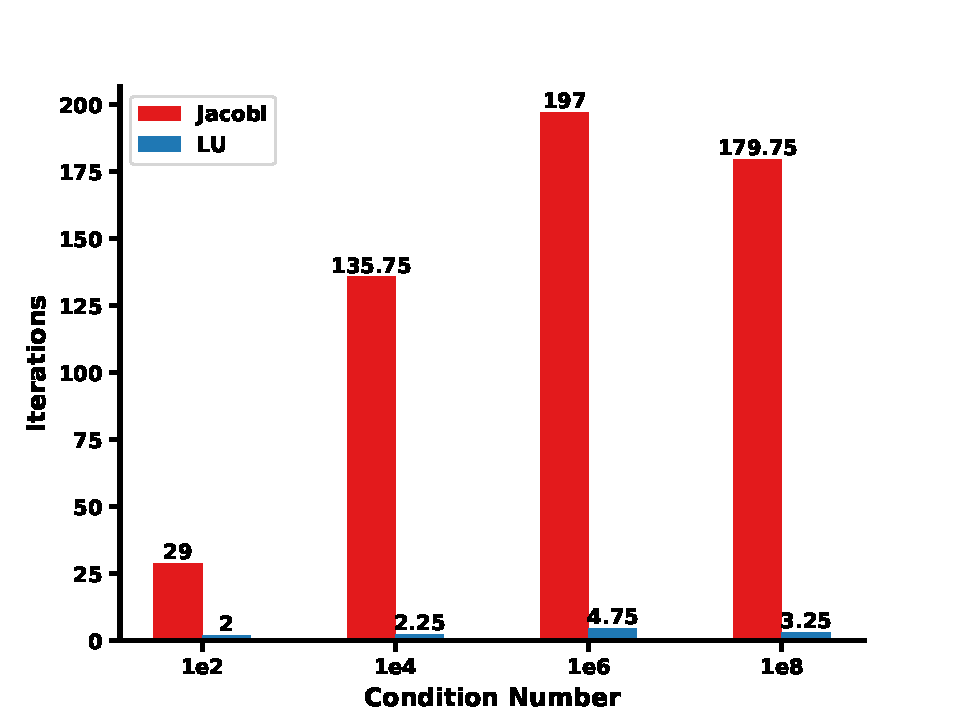
\includegraphics[width=0.7\linewidth]{chapters/5_experiments/figures/LR_iter.pdf}
    \caption[Low-Rank IR - GMRES Iterations]{Comparison of diagonal and LU preconditioning for $1024 \times 1024$ matrices with varying condition number. The iteration count is given as the average across all accuracy settings (i.e. $\epsilon$)}
    \label{fig:lr_ir_iter}
\end{figure}

Since each GMRES iteration is comparatively expensive due to the matrix-vector products computed in high-precision, there is a direct transfer from a reduction of the iteration count to a decrease in runtime. This becomes immediately evident when comparing the total time necessary to produce an accurate solution. For this experiment, every routine has been executed $10$ times, taking the average to produce the numbers shown in Figure~\hyperref[fig:lr_ir_iter]{\ref{fig:lr_ir_iter}}. Diagonal (Jacobi) preconditioning is never able to outperform the hierarchical LU factors, due to the high iteration count (and the aforementioned reasons). 

The performance of LU- and GMRES-based iterative refinement, on the other hand, seems to be almost identical for the illustrated settings, but are actually dependent on the condition number and the factorization accuracy. In the figure, LU-based IR takes approximately 6 iterations to converge, while GMRES-based IR only takes one. Again, the high precision calculation inside the GMRES calculation are largely responsible for the difference in runtime for a single step. If the gap in iteration count between those two methods increases (either via a higher condition number or a lower $\epsilon$, see Figures~\hyperref[fig:lrir1]{\ref{fig:lrir1}} - \hyperref[fig:lrir4]{\ref{fig:lrir4}}), GMRES-based IR becomes more favourable. However, as long as the number of necessary iterations remains low, LU-based IR is definitely preferable due to its faster runtime. In the current implementation, it has the additional advantage that it does not require the preconditioner to be applied in high-precision and can thus profit from the reduced complexity of a hierarchical triangular solve (which is not available in high-precision). Due to the small matrix sizes employed, it is not expected to have a huge impact on the measurements, but it should be mentioned nonetheless.

\begin{figure}[h]
    \centering
    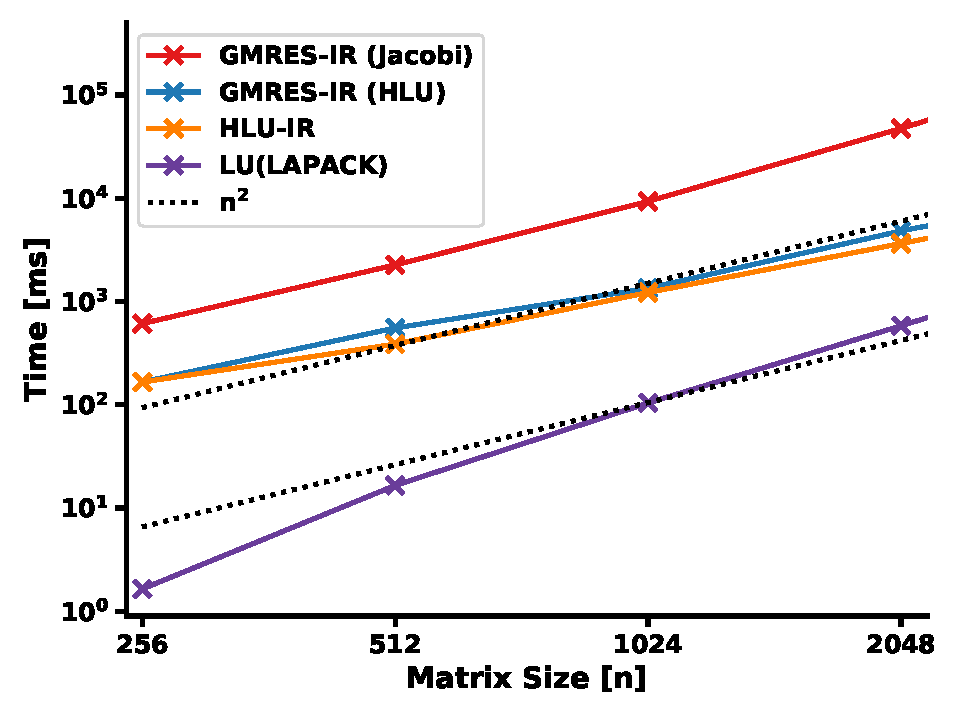
\includegraphics[width=0.7\linewidth]{chapters/5_experiments/figures/LR_scaling.pdf}
    \caption[Low-Rank IR - Runtime]{Comparison of different low-rank IR methods and a direct solver via dense LU factorization ($\kappa_\infty(A)=10^8$ and $\epsilon = 10^{-4}$ for all matrices).}
    \label{fig:lr_ir_scaling}
\end{figure}

Furthermore, the number of iterations necessary for LU-based IR can be directly controlled via the parameter $\epsilon$. In the set of test matrices used, decreasing this accuracy threshold by a factor of $10^{-2}$, typically only increased the rank by a small amount($+2$ or $+3$). The high performance of hierarchical formats is based on the assumption that $rank \ll n$ and the influence of such a slight increase might be negligible. Thus, if a higher accuracy can be achieved without deteriorating the efficiency of the hierarchical format, LU-based IR is expected to outperform GMRES for almost all settings. However, further research and experiments are necessary to investigate this hypothesis.

Finally, the graph in Figure~\hyperref[fig:lr_ir_iter]{\ref{fig:lr_ir_iter}} also serves to demonstrate that the proposed approach is not beneficial for small matrix sizes. Due to the highly optimized linear algebra kernels available (e.b. BLAS, LAPACK), direct solving via LU factorization can be done very performance efficient. Indeed for $n \leq 4096$, no advantage in runtime can be observed for the proposed methods. Even though, the scaling of the methods is inarguably different, with both LU- and GMRES-based iterative refinement exhibiting a complexity of $\mathcal{O}(n^2)$, while direct solving clearly surpasses that threshold (and in fact, is known to scale with $\mathcal{O}(n^3)$). Therefore, iterative refinement based on low-rank approximations becomes increasingly attractive for larger matrices, promising to achieve equal results while being an order of magnitude faster.



